A buried cable has stopped working. A technician sends a short voltage pulse into it and records the voltage at its start (see graph): the pulse, and later its echo from the fault. Pulses run along the cable at \vsO.

\begin{center}
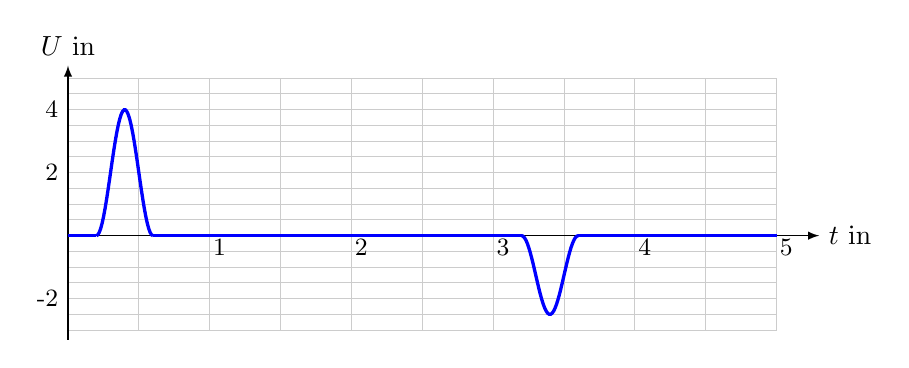
\begin{tikzpicture}[>=latex, x=1.8cm, y=0.4cm]
 \draw[gray!40, step=0.5] (0,-3) grid (5,5);
 \draw[->] (0,0) -- (5.3,0) node[right] {$t$ in \si{\micro\s}};
 \draw[->] (0,-3.3) -- (0,5.4) node[above] {$U$ in \si{\V}};
 \foreach \t in {1,2,3,4,5} \node[below right, inner sep=1pt] at (\t,0) {\small \t};
 \foreach \u in {-2,2,4} \node[left] at (0,\u) {\small \u};
 \draw[very thick, blue] (0,0) -- (0.2,0);
 \draw[very thick, blue, domain=0.2:0.6, samples=40] plot (\x, {4*sin(deg(pi*(\x-0.2)/0.4))^2});
 \draw[very thick, blue] (0.6,0) -- (3.2,0);
 \draw[very thick, blue, domain=3.2:3.6, samples=40] plot (\x, {-2.5*sin(deg(pi*(\x-3.2)/0.4))^2});
 \draw[very thick, blue] (3.6,0) -- (5,0);
\end{tikzpicture}
\end{center}

\begin{abcliste}
\abc How far from the start of the cable is the fault?

\abc Is it a break (an open end) or a short circuit? Explain.
\end{abcliste}
